\documentclass{article}
\usepackage{graphicx} % Required for inserting images
\usepackage{float}
\usepackage{color}
\usepackage{hyperref}
\usepackage{multicol}
\usepackage{scalerel}
\usepackage[
	citestyle=ieee, 
    bibstyle=ieee,
    style=numeric-comp,
    sorting=nty,
    maxbibnames=99, % Make sure we are printing all authors in the appendix
]{biblatex}
\addbibresource{references.bib}

\usepackage{booktabs}
\usepackage{anysize}
\usepackage{caption}
\usepackage[toc,page]{appendix}
\usepackage{subcaption}
\usepackage{fancyhdr}
\usepackage{amssymb}
\usepackage{amsmath}
\usepackage{pgffor} % Allows using foreach

\pagestyle{plain}
\oddsidemargin  -5mm
\evensidemargin -5mm
\topmargin      -5mm
\textwidth      170mm
\textheight     225mm
\parskip    1.5ex
\parindent   0cm
\footskip 15mm
\usepackage{datetime}
\usepackage{bm}
\pagestyle{fancy}
\fancyhf{}

\chead{CSN \hfill Lab Session 7 –Simulation of SIS model over networks \hfill Daniel Benedí Garcia \& Dídac Martínez Bachs}
\setlength{\headheight}{13.07225pt}
\newcommand{\imgHeight}{1.2}

\newcommand{\param}[1]{\ensuremath{\vec{\bm{#1}}}}

\newdateformat{monthyeardate}{%
  \monthname[\THEMONTH], \THEYEAR}

\title{Complex and Social Networks \\ Assignment 7 - Simulation of SIS model over networks}
\author{Daniel Benedí Garcia \\ Dídac Martínez Bachs}
\date{\monthyeardate\today}

%\title{LAB7}
%\author{Daniel Benedí Garcia \& Dídac Martínez Bachs}
%\date{December 2023}
\begin{document}

%\maketitle
\begin{multicols}{2}
\tableofcontents
\end{multicols}
\hrule
\section{Introduction}
Centrality measures play a pivotal role in network analysis, as they help identify the most influential and well-connected nodes. Closeness centrality, in particular, offers a unique perspective by quantifying how easily information can flow from a node to all other nodes in the network. Its application to syntactic dependency networks (SDN) allows the study of the significance of words in conveying information, their role in sentence comprehension, and their impact on language processing and generation. See a representation of a SDN in Figure \ref{fig:sdn}.

To facilitate the computation of closeness centrality in SDN, this paper introduces the utilization of two distinct models based on two hypohteses. 
\begin{enumerate}[I]
    \item The measure of closeness centrality in syntactic dependency networks is significantly modeled by binomial (Erdos-Renyi) graphs, keeping the original numbers of edges and vertices.
    \item The measure of closeness centrality in syntactic dependency networks is significantly modeled by randomized graphs preserving the original degree sequence. The model depends on the original list of edges and a parameter $Q$ governing the repetitions of the random graph generation.
\end{enumerate}

These models offer a more efficient computational approach to evaluating closeness centrality while preserving the essential structural characteristics of the original networks.

The report studies the significance of the closeness centrality metrics obtained through these models in comparison to the original syntactic dependency networks. We seek to analyze how the metrics derived from the binomial (I) and degree-preserving random graph (II) models compare to those from the original networks. By doing so, we aim to tackle whether these simplified representations offer meaningful insights and faithfully capture the centrality of words in sentence structures.

This document is strucutred in four different sections. Next, results are presented in section \ref{sec:results}. Discussion and conclusions are covered in section \ref{sec:discussion}, and finally, some aspects of the methodology are presented in section \ref{sec:methods}.

\begin{figure}
    \centering
    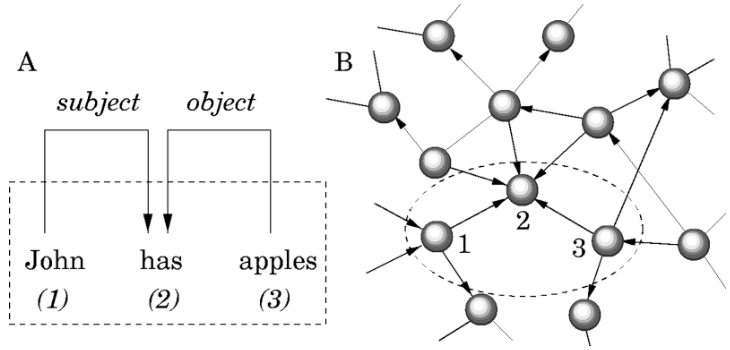
\includegraphics[width=0.5\textwidth]{figures/sdn.png}
    \caption{(a) The syntactic structure of a simple sentence. Here words define the nodes in a graph and the binary relations (arcs) represent syntactic dependencies. Here we assume arcs go from modifier to its head. The proper noun “John” and the verb “has” are syntactically dependent in the sentence. John is a modifier of the verb has, which is its head. Similarly, the action of has is modified by its object “apples.” (b) Mapping the syntactic dependency structure of the sentence in (a) into a global syntactic dependency network. Extracted from \cite{i2004patterns}}
    \label{fig:sdn}
\end{figure}

\section{First Exercise}
\subsection{Methodology}
We will study the behaviour of the evolution of an epidemic on graphs constructed using the following five different models:
\begin{itemize}
\item Erdös-Renyi model
\item Barabási-Albert model
\item Small-World or Watts-Strogatz model
\item Star
\item Tree
\end{itemize}

Two sets of experiments have been carried out.
\begin{itemize}
\item The first experiment consisted of plotting the spread of the epidemic with a recovery probability of $\gamma = 0.30$, a spread probability of $\beta = 0.40$ and different percentages of infected nodes initially, $p_0 \in \{0.1,0.25, 0.5, 0.75, 0.9\}$. Then we compared the result obtained with the leading eigenvalue for each network.
\item In the second experiment, we try to observe the variability of the leading eigenvalues on nondeterministic random networks in order to validate the results obtained in the previous experiment and the following task. 
\end{itemize}

All experiments have been performed with 10 repetitions in order to reduce the noise produced by the random nature of the epidemic simulation.

In order to improve the performance of the simulation, instead of spreading from the infectious nodes to the susceptible nodes, we checked what the probability of a node being infected given the number of infectious neighbors is. It was obtained from the following formula:
\begin{align*}
    P(v_{t+1} = \text{Infected}| v_{t} = \text{Susceptible}) &= \bigcup_{u \in N(v)} P(Spread of u_t) \\
    &= 1 - \bigcap_{u \in N(v)} 1 - P(Spread of u_t) \\
    &= 1 - (1-\beta)^{|N(v)\cap \text{Infected}|}
\end{align*}
That means that we can simply know the probability of a node to get infected by knowing how many of its neighbours are infected. 

\subsection{Results}
In figure \ref{fig:all_networks}, we can observe how all the tested networks evolve with an initial proportion of 25\% of the infected nodes. In Appendix \ref{Appendix:AllNetworks}, we can observe the same results of the experiments, but with a percentage of 10\%, 25\%, 50\%, 75\% and 90\%.

\begin{figure}
    \centering
    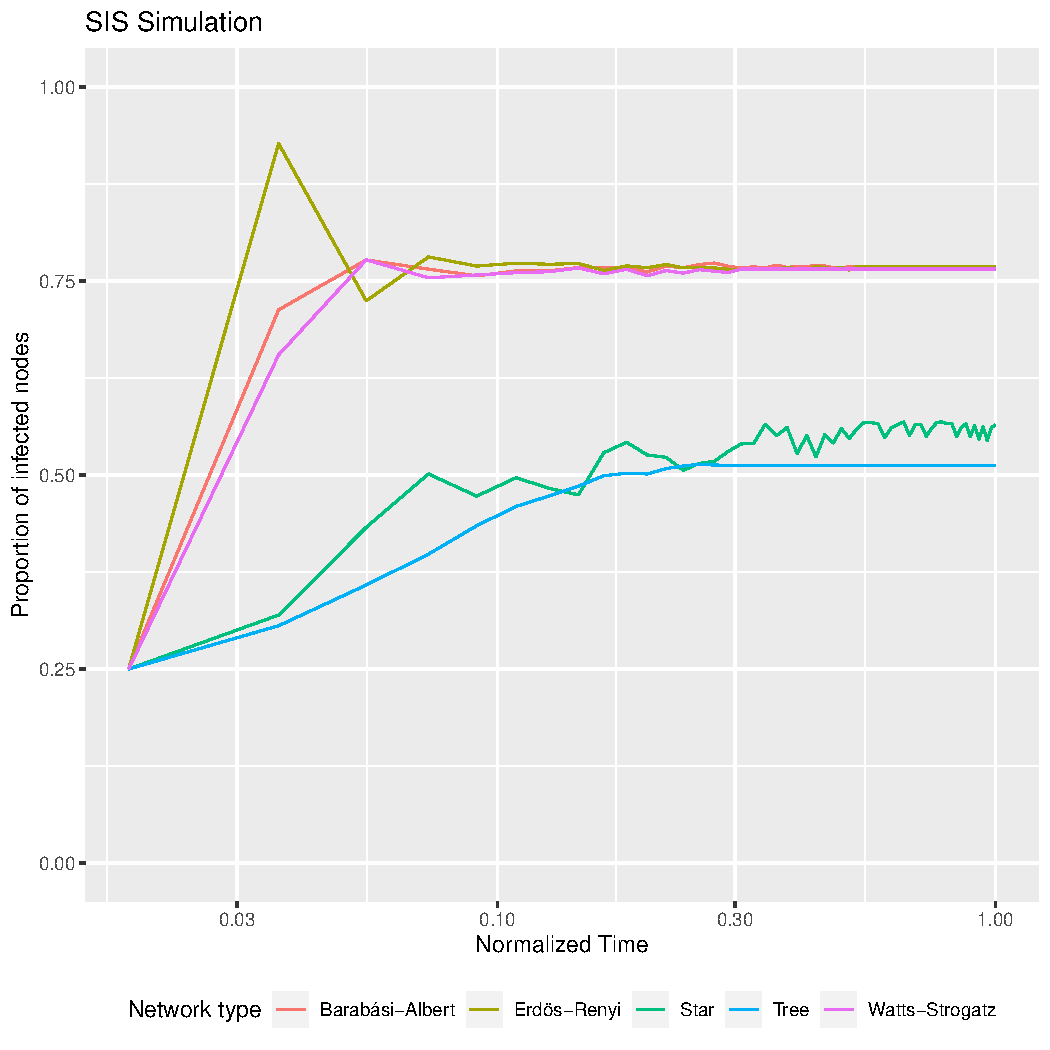
\includegraphics[width=0.4\textwidth]{img/AllNetworks_0.25.pdf}
    \caption{Evolution of the spread for all the tested networks with $\gamma = 0.30, \beta = 0.40, p_0=0.25$}
    \label{fig:all_networks}
\end{figure}

We can observe that in all networks the pandemic continues to spread until it reaches a saturation point. This saturation point does not depend on the initial proportion of infected nodes, as can be seen in the Appendix \ref{Appendix:AllNetworks}. If we observe the leading eigenvalue of each network (Table \ref{tab:eigens}), our beta is always above all thresholds, and therefore we expected to have a pandemic. It is remarkable that Erdös-Renyi, Barbási-Albert, and Watts-Strogatz have a faster start than the Star and Tree networks. We could not relate this behavior to the leading eigenvalue because the Star network has a higher eigenvalue than Watts-Strogatz, but it does not have a faster start. 

% latex table generated in R 4.2.0 by xtable 1.8-4 package
% Thu Dec 28 11:33:35 2023
\begin{table}[ht]
\centering
\begin{tabular}{lrr}
  \hline
Network & Leading Eigenvalue & Threshold \\ 
  \hline
Erdös-Renyi & 399.5150002 & 0.00075091 \\ 
  Barabási-Albert & 29.9042477 & 0.01003202 \\ 
  Watts-Strogatz & 10.4933208 & 0.02858961 \\ 
  Tree & 3.5769977 & 0.08386922 \\ 
  Star & 31.6069613 & 0.00949158 \\ 
   \hline
\end{tabular}
\caption{Leading Eigenvalues of each network and the threshold for beta \label{tab:eigens}}
\end{table}


Because the threshold for beta depends on the leading eigenvalue, which depends on the network, we studied how much it varies. In Appendix \ref{Appendix:Eigens}, we show the boxplot of several repetitions in which we generated a graph and checked its leading eigenvalue. First, we observe that all the eigenvalues have a small variation, which allows us to corroborate the previous results. Moreover, we found remarkable that the leading eigenvalue in Erdös-Renyi networks is very close to the expected number of vertices, with really little variation. We also found interesting that the number of children per node in a Tree network does not vary the leading eigenvalues.

\section{Second Exercise}
\subsection{Methodology}
We have modeled the evolution of an epidemic spread for the same kind of network as in the previous task. For all of them, we have plotted the evolution of the epidemic when the relation between $\beta$, $\gamma$ is slightly above and below the theoretical epidemic threshold. The theoretical epidemic threshold states whether the infection dies out over time or survives and becomes an epidemic. Chakrabarti et al. empirically observed in \cite{Chakrabarti2008} that such a relation is indeed: 
$$
    \frac{\beta}{\gamma} = \frac{1}{\lambda_1}
$$
with $\lambda_1$ being the leading eigenvalue. Therefore, we have fixed some values of $\gamma$ and calculated $\beta = \frac{\beta}{\lambda_1} + \varepsilon, \varepsilon\in\{-0.05,0.05\}$, in order to analyze whether the epidemic threshold was the expected one for each network. Because, if the relation is above, we expect the epidemic to occur; and if the relation is below, we expect no epidemic to occur.

Moreover, we have used a set of different values for $\gamma$ and the parameters that allow us to define the different networks such as:
\begin{itemize}
    \item In the Erdös-Renyi model, the expected density
    \item In the Barbási-Albert model, the number of clusters
    \item In the Watts-Strogatz model, the rewiring probability
    \item In the Tree model, the number of children per node
\end{itemize}

The set of values used for $\gamma$ are:
$$
    \gamma \in \{ 0.15, 0.3, 0.45, 0.6, 0.75, 0.9 \}
$$

All experiments have been performed with 10 repetitions in order to reduce the noise produced by the random nature of the epidemic simulation.

\subsection{Results}
In the following appendices, we present the outcomes obtained from various network models. Specifically, Appendix \ref{Appendix:ErdosRenyi} showcases the results from the Erdös-Renyi model, while Appendix \ref{Appendix:BarabasiAlbert} displays the outcomes from the Barbäsi-Albert model. Additionally, Appendix \ref{Appendix:SmallWorld} provides the results for the Watts-Strogatz model, Appendix \ref{Appendix:Star} presents the outcomes of the Star model, and Appendix \ref{Appendix:Tree} exhibits the results for the Tree model.

Results show that, in general, in the first case (case where the previously mentioned relation is slightly higher than threshold), the number of infected nodes grows until it reaches a stabilization point, meaning that the infection becomes an epidemic with a stable rate of infected nodes or saturation point, which is different for each type of graph, while in the second case (case where the previously mentioned relation is slightly lower than threshold) shows that the number of infected nodes drops to zero, meaning the infection dies and therefore does not turn into an epidemic. 

This behavior can be observed for all values of $\gamma$ and different configurations of the networks that have been used in these experiments, supporting the existence of this theoretical threshold in complex networks such as those that define social interconnections in real life.

From plots in \ref{Appendix:ErdosRenyi}, \ref{Appendix:BarabasiAlbert} and \ref{Appendix:SmallWorld}, one can observe that the higher $\gamma$, the less time it takes to reach the death point of the infection, when we are below the epidemic threshold. However, the higher $\gamma$, the longer it takes to reach equilibrium or convergence in the number of infected nodes, and a higher number of infected nodes will be required to reach the expected saturation point. Additionally, it is worth mentioning that as the value of $\gamma$ increases, the equilibrium point decreases. On the other hand, we observed that the magnitude of the leading eigenvector does not seem to be as determinant as $\gamma$.

The deterministic models of graph generation demonstrate a similar behavior to the random models in terms of the spread of the epidemic. The epidemic threshold can be determined from the plots in Appendix \ref{Appendix:Star} and Appendix \ref{Appendix:Tree}. These plots indicate that the networks generated using deterministic models tend to restrict the spread of infections to a smaller expected number of infected nodes. This can be attributed to the specific structural properties of these graphs, leading to different patterns of epidemic spread. 

In a tree graph, the absence of cycles implies a hierarchical structure with a unique path from the root to any node. This hierarchical arrangement often results in a linear spread of infection. Each node in the tree has only one direct path to the source of infection, and, as a consequence, the infection tends to spread linearly along the branches of the tree, causing a smaller percentage of infected nodes (almost zero when the recovery probability is high). Furthermore, since nodes in a tree have fewer connections compared to random graphs, the potential for widespread transmission is limited. This results in a slower and more localized epidemic spread. 

In a star graph, all peripheral nodes are directly connected to a central node. The central node plays an important role in the transmission of infection to the periphery. The infection can spread only through two routes: from the central node to the peripheral nodes and vice versa. This limited set of transmission routes restricts the overall spread of the epidemic.

From these observations some interesting conclusions can be inferred:
\begin{itemize}
\item The experimental validation of the theoretical epidemic threshold demonstrates its existence across a range of graphs, created through the use of either random  or deterministic models. Notably, there is no discernible difference between these graph types in terms of the existence of an epidemic threshold, as all consistently manifest its inherent presence due to obvious behavior differences, such as infection's extinction when experiments have taken place below this threshold or infection evolution into epidemic when experiments have taken place above this threshold.
\item In the context of infection dynamics, the relation between $\gamma$ and $\beta$ plays a predominant role, overshadowing the impact of the configuration of the type of network.
\item Structural characteristics of tree and star graphs, such as linear spread in trees and centralized connectivity in stars, contribute to a more localized and constrained epidemic spread compared to the more interconnected and random nature of graphs like Erdös-Renyi, Barabási-Albert, and Watts-Strogatz. These insights into the relationship between graph structure and epidemic dynamics are valuable for understanding how network topology influences the transmission of infectious diseases and can inform strategies for disease control and prevention.

\end{itemize}

\printbibliography

\pagebreak
\appendix
\def\Languages{
Arabic, Basque, Catalan,
Chinese, Czech, English,
Greek, Hungarian, Italian,
Turkish}

\section{Graphs of all the models for each language}\label{appendix:plots}

\foreach \lang in \Languages
{
\begin{figure}[!htb]
    \centering
    \includegraphics[width=0.7\textwidth]{figures/\lang_all_models.pdf}
    \caption{All models fitted for \lang}
\end{figure}
}
\pagebreak

\section{The best model by AIC for each language}\label{appendix:best-model-plots}

\foreach \lang in \Languages
{
\begin{figure}[!htb]
    \centering
    \includegraphics[width=0.7\textwidth]{figures/\lang_best_aic.pdf}
    \caption{The best model for \lang}
\end{figure}
}
\pagebreak

\section{The best model by $s$ for each language}

\foreach \lang in \Languages
{
\begin{figure}[!htb]
    \centering
    \includegraphics[width=0.7\textwidth]{figures/\lang_best_s.pdf}
    \caption{The best model for \lang}
\end{figure}
}
\pagebreak

\section{Data Samples provided for each language \label{appendix:data_samples}}
\foreach \lang in \Languages
{
\begin{figure}[!htb]
    \centering
    \includegraphics[width=0.7\textwidth]{figures/\lang_dataset.pdf}
    \caption{Data Samples for \lang}
\end{figure}
}
\pagebreak

\section{Weighted Nonlinear Least Squares \label{appendix:weighted}}

\foreach \lang in \Languages
{
\begin{figure}[!htb]
    \centering
    \begin{subfigure}{0.4\textwidth}
        \includegraphics[width=\textwidth]{figures/\lang_best_aic_weighted.pdf}
        \caption{Model with smallest AIC for \lang.}
    \end{subfigure} \hfill
    \begin{subfigure}{0.4\textwidth}
        \includegraphics[width=\textwidth]{figures/\lang_best_s_weighted.pdf}
        \caption{Models with smallest $s$ \lang.}
    \end{subfigure}
    \caption{Models fitted for language \lang}
\end{figure}
\begin{figure}[!htb]
    \centering
    \includegraphics[width=0.7\textwidth]{figures/\lang_all_models_weighted.pdf}
    \caption{All models for language \lang.}
\end{figure}
}

\begin{table}[!htb]
\centering
\resizebox{\columnwidth}{!}{
\begin{tabular}{llllllllllll}
Language & 0 & 1 & 2 & 3 & 4 & 5 & 1+ & 2+ & 3+ & 4+ & 5+ \\ \hline

 Arabic & 1090.844 & 235.935 & 235.521 & 275.158 & 268.201 & 224.634 & 236.397 & 231.094 & 274.438 & 266.068 & 241.632 \\
 Basque & 276.863 & 32.845 & 32.396 & 64.283 & 49.796 & 33.756 & 32.756 & 33.646 & 89.041 & 50.941 & 35.646 \\
 Catalan & 814.121 & 35.646 & 32.216 & 148.302 & 98.362 & 28.594 & 33.100 & 31.855 & 154.736 & 90.916 & 35.415 \\
 Chinese & 274.712 & 89.864 & 88.606 & 88.801 & 97.953 & 85.676 & 89.439 & 87.615 & 87.605 & 99.951 & 102.902 \\
 Czech & 723.596 & 428.590 & 421.061 & 424.942 & 439.635 & 416.160 & 426.906 & 411.535 & 413.922 & 440.122 & 418.808 \\
 English & 724.102 & 152.683 & 154.417 & 247.931 & 184.732 & 155.759 & 154.457 & 156.371 & 257.720 & 185.313 & 183.950 \\
 Greek & 711.355 & 156.227 & 155.661 & 193.590 & 173.208 & 156.703 & 156.055 & 156.800 & 205.467 & 173.253 & 158.695 \\
 Hungarian & 610.872 & 143.952 & 143.565 & 274.453 & 269.788 & 145.511 & 143.633 & 145.551 & 265.868 & 241.818 & 147.481 \\
 Italian & 705.677 & 134.719 & 128.651 & 173.938 & 160.282 & 122.408 & 130.492 & 124.636 & 175.543 & 161.160 & 124.370 \\
 Turkish & 412.776 & 20.871 & 19.327 & 96.241 & 49.615 & 20.250 & 19.339 & 21.317 & 110.629 & 50.554 & 17.680 \\
\end{tabular}}
\caption{Akaike information criterion (AIC) of each model \label{tab:aic}}
\end{table}

\begin{table}[!htb]
\centering
\resizebox{\columnwidth}{!}{
\begin{tabular}{llllllllllll}
Language & 0 & 1 & 2 & 3 & 4 & 5 & 1+ & 2+ & 3+ & 4+ & 5+ \\ \hline

 Arabic & 866.211 & 11.301 & 10.888 & 50.525 & 43.567 & 0.000 & 11.764 & 6.460 & 49.805 & 41.434 & 16.998 \\
 Basque & 244.467 & 0.449 & 0.000 & 31.887 & 17.400 & 1.360 & 0.360 & 1.250 & 56.646 & 18.545 & 3.250 \\
 Catalan & 785.527 & 7.052 & 3.621 & 119.708 & 69.767 & 0.000 & 4.506 & 3.261 & 126.141 & 62.322 & 6.820 \\
 Chinese & 189.036 & 4.188 & 2.931 & 3.126 & 12.277 & 0.000 & 3.763 & 1.939 & 1.929 & 14.275 & 17.227 \\
 Czech & 312.061 & 17.055 & 9.527 & 13.408 & 28.100 & 4.625 & 15.371 & 0.000 & 2.388 & 28.587 & 7.274 \\
 English & 571.419 & 0.000 & 1.734 & 95.248 & 32.049 & 3.076 & 1.774 & 3.688 & 105.037 & 32.630 & 31.267 \\
 Greek & 555.693 & 0.566 & 0.000 & 37.928 & 17.546 & 1.042 & 0.393 & 1.138 & 49.806 & 17.592 & 3.033 \\
 Hungarian & 467.306 & 0.387 & 0.000 & 130.887 & 126.223 & 1.945 & 0.068 & 1.986 & 122.302 & 98.252 & 3.916 \\
 Italian & 583.268 & 12.310 & 6.243 & 51.530 & 37.874 & 0.000 & 8.084 & 2.227 & 53.135 & 38.752 & 1.962 \\
 Turkish & 395.096 & 3.191 & 1.647 & 78.561 & 31.935 & 2.570 & 1.659 & 3.636 & 92.949 & 32.874 & 0.000 \\
\end{tabular}}
\caption{AIC differences \label{tab:aic_diff}}
\end{table}

\begin{table}[!htb]
\centering
\resizebox{\columnwidth}{!}{
\begin{tabular}{llllllllllll}
Language & 0 & 1 & 2 & 3 & 4 & 5 & 1+ & 2+ & 3+ & 4+ & 5+ \\ \hline

 Arabic & 22.599 & 0.044 & 0.044 & 0.052 & 0.050 & 0.042 & 0.044 & 0.043 & 0.051 & 0.050 & 0.045 \\
 Basque & 6.380 & 0.044 & 0.043 & 0.063 & 0.054 & 0.044 & 0.044 & 0.044 & 0.084 & 0.054 & 0.044 \\
 Catalan & 16.624 & 0.023 & 0.022 & 0.041 & 0.031 & 0.022 & 0.022 & 0.022 & 0.042 & 0.030 & 0.022 \\
 Chinese & 6.219 & 0.087 & 0.085 & 0.085 & 0.096 & 0.081 & 0.086 & 0.083 & 0.083 & 0.097 & 0.098 \\
 Czech & 14.600 & 0.225 & 0.214 & 0.219 & 0.239 & 0.207 & 0.221 & 0.202 & 0.204 & 0.239 & 0.209 \\
 English & 14.642 & 0.047 & 0.047 & 0.080 & 0.056 & 0.047 & 0.047 & 0.047 & 0.084 & 0.056 & 0.055 \\
 Greek & 14.958 & 0.050 & 0.049 & 0.061 & 0.055 & 0.049 & 0.049 & 0.049 & 0.065 & 0.054 & 0.049 \\
 Hungarian & 10.376 & 0.051 & 0.050 & 0.112 & 0.110 & 0.050 & 0.050 & 0.050 & 0.106 & 0.092 & 0.051 \\
 Italian & 15.185 & 0.044 & 0.043 & 0.056 & 0.052 & 0.041 & 0.043 & 0.041 & 0.056 & 0.052 & 0.041 \\
 Turkish & 8.885 & 0.030 & 0.030 & 0.058 & 0.039 & 0.030 & 0.030 & 0.030 & 0.066 & 0.039 & 0.029 \\
\end{tabular}}
\caption{Residual standard error for each model \label{tab:res_se}}
\end{table}

\begin{table}[!htb]
\centering
\resizebox{\columnwidth}{!}{
\begin{tabular}{llllllllllllllllllllllll}
         & \multicolumn{23}{l}{Model} \\ \cline{2-24} 
         & \multicolumn{1}{l|}{1} & \multicolumn{2}{l|}{2}     & \multicolumn{2}{l|}{3}     & \multicolumn{1}{l|}{4} & \multicolumn{1}{l|}{5}         & \multicolumn{2}{l|}{1+}    & \multicolumn{3}{l|}{2+}        & \multicolumn{3}{l|}{3+}        & \multicolumn{2}{l}{4+} & \multicolumn{4}{l}{5+} \\
Language & \multicolumn{1}{l|}{b} & a & \multicolumn{1}{l|}{b} & a & \multicolumn{1}{l|}{c} & \multicolumn{1}{l|}{a} & a & b & \multicolumn{1}{l|}{c} & b & \multicolumn{1}{l|}{d} & a & b & \multicolumn{1}{l|}{d} & a & c & \multicolumn{1}{l|}{d} & a & d \\ \hline

 Arabic & \multicolumn{1}{l|}{0.339} & 0.708 & \multicolumn{1}{l|}{0.367} & 1.531 & \multicolumn{1}{l|}{0.009} & \multicolumn{1}{l|}{0.773} & 0.888 & 0.252 & \multicolumn{1}{l|}{0.003} & 0.348 & \multicolumn{1}{l|}{-0.080} & 0.200 & 0.601 & \multicolumn{1}{l|}{0.799} & 35.108 & 0.001 & \multicolumn{1}{l|}{-33.756} & 0.700 & 0.232  & 1.812 & 0.143 & 0.003 & \multicolumn{1}{l|}{-1.030}\\
 Basque & \multicolumn{1}{l|}{0.432} & 0.661 & \multicolumn{1}{l|}{0.468} & 1.312 & \multicolumn{1}{l|}{0.028} & \multicolumn{1}{l|}{0.922} & 0.707 & 0.420 & \multicolumn{1}{l|}{0.003} & 0.445 & \multicolumn{1}{l|}{-0.091} & 0.424 & 0.567 & \multicolumn{1}{l|}{0.345} & 18.722 & 0.002 & \multicolumn{1}{l|}{-17.646} & 0.875 & 0.118  & 0.423 & 0.567 & -0.000 & \multicolumn{1}{l|}{0.346}\\
 Catalan & \multicolumn{1}{l|}{0.351} & 0.720 & \multicolumn{1}{l|}{0.374} & 1.456 & \multicolumn{1}{l|}{0.012} & \multicolumn{1}{l|}{0.794} & 0.787 & 0.324 & \multicolumn{1}{l|}{0.002} & 0.359 & \multicolumn{1}{l|}{-0.070} & 0.476 & 0.449 & \multicolumn{1}{l|}{0.342} & 17.843 & 0.001 & \multicolumn{1}{l|}{-16.533} & 0.723 & 0.218  & 1.882 & 0.170 & 0.003 & \multicolumn{1}{l|}{-1.183}\\
 Chinese & \multicolumn{1}{l|}{0.442} & 0.559 & \multicolumn{1}{l|}{0.530} & 1.199 & \multicolumn{1}{l|}{0.032} & \multicolumn{1}{l|}{0.927} & 0.813 & 0.263 & \multicolumn{1}{l|}{0.017} & 0.469 & \multicolumn{1}{l|}{-0.192} & 0.109 & 0.929 & \multicolumn{1}{l|}{0.828} & 15.477 & 0.005 & \multicolumn{1}{l|}{-14.535} & 0.931 & -0.010  & 0.894 & 0.253 & 0.011 & \multicolumn{1}{l|}{-0.179}\\
 Czech & \multicolumn{1}{l|}{0.471} & 0.158 & \multicolumn{1}{l|}{0.864} & 1.703 & \multicolumn{1}{l|}{0.015} & \multicolumn{1}{l|}{1.013} & 0.567 & 0.412 & \multicolumn{1}{l|}{0.008} & 0.515 & \multicolumn{1}{l|}{-0.600} & 0.007 & 1.550 & \multicolumn{1}{l|}{1.223} & 8.684 & 0.007 & \multicolumn{1}{l|}{-7.779} & 1.238 & -0.677  & 0.000 & 2.360 & -0.007 & \multicolumn{1}{l|}{1.328}\\
 English & \multicolumn{1}{l|}{0.456} & 0.754 & \multicolumn{1}{l|}{0.447} & 1.862 & \multicolumn{1}{l|}{0.013} & \multicolumn{1}{l|}{1.063} & 0.794 & 0.420 & \multicolumn{1}{l|}{0.001} & 0.453 & \multicolumn{1}{l|}{0.031} & 0.817 & 0.432 & \multicolumn{1}{l|}{-0.092} & 34.841 & 0.001 & \multicolumn{1}{l|}{-33.341} & 1.114 & -0.155  & 3.937 & 0.128 & 0.002 & \multicolumn{1}{l|}{-3.421}\\
 Greek & \multicolumn{1}{l|}{0.358} & 0.685 & \multicolumn{1}{l|}{0.393} & 1.423 & \multicolumn{1}{l|}{0.014} & \multicolumn{1}{l|}{0.800} & 0.747 & 0.345 & \multicolumn{1}{l|}{0.002} & 0.370 & \multicolumn{1}{l|}{-0.107} & 0.402 & 0.494 & \multicolumn{1}{l|}{0.409} & 17.421 & 0.001 & \multicolumn{1}{l|}{-16.162} & 0.741 & 0.176  & 0.633 & 0.381 & 0.002 & \multicolumn{1}{l|}{0.132}\\
 Hungarian & \multicolumn{1}{l|}{0.593} & 0.605 & \multicolumn{1}{l|}{0.617} & 2.078 & \multicolumn{1}{l|}{0.020} & \multicolumn{1}{l|}{1.509} & 0.594 & 0.626 & \multicolumn{1}{l|}{-0.000} & 0.598 & \multicolumn{1}{l|}{-0.103} & 0.621 & 0.611 & \multicolumn{1}{l|}{-0.031} & 43.430 & 0.002 & \multicolumn{1}{l|}{-42.110} & 1.940 & -1.277  & 0.540 & 0.652 & -0.001 & \multicolumn{1}{l|}{0.084}\\
 Italian & \multicolumn{1}{l|}{0.359} & 0.632 & \multicolumn{1}{l|}{0.416} & 1.434 & \multicolumn{1}{l|}{0.013} & \multicolumn{1}{l|}{0.797} & 0.771 & 0.308 & \multicolumn{1}{l|}{0.004} & 0.378 & \multicolumn{1}{l|}{-0.159} & 0.202 & 0.644 & \multicolumn{1}{l|}{0.697} & 31.214 & 0.001 & \multicolumn{1}{l|}{-30.029} & 0.755 & 0.126  & 1.137 & 0.235 & 0.004 & \multicolumn{1}{l|}{-0.400}\\
 Turkish & \multicolumn{1}{l|}{0.412} & 0.686 & \multicolumn{1}{l|}{0.439} & 1.399 & \multicolumn{1}{l|}{0.021} & \multicolumn{1}{l|}{0.900} & 0.645 & 0.479 & \multicolumn{1}{l|}{-0.002} & 0.422 & \multicolumn{1}{l|}{-0.082} & 0.709 & 0.433 & \multicolumn{1}{l|}{-0.032} & 14.405 & 0.003 & \multicolumn{1}{l|}{-13.249} & 0.866 & 0.094  & 0.141 & 0.957 & -0.013 & \multicolumn{1}{l|}{0.721}\\
\end{tabular}}
\caption{Parameters of each fitted model \label{tab:params}}
\end{table}




\end{document}
